%% Copernicus Publications Manuscript Preparation Template for LaTeX Submissions
%% ---------------------------------
%% This template should be used for copernicus.cls
%% The class file and some style files are bundled in the Copernicus Latex Package, which can be downloaded from the different journal webpages.
%% For further assistance please contact Copernicus Publications at: production@copernicus.org
%% https://publications.copernicus.org/for_authors/manuscript_preparation.html

%% copernicus_rticles_template (flag for rticles template detection - do not remove!)

%% Please use the following documentclass and journal abbreviations for discussion papers and final revised papers.

%% 2-column papers and discussion papers
\documentclass[gmd, manuscript]{copernicus}



%% Journal abbreviations (please use the same for preprints and final revised papers)

% Advances in Geosciences (adgeo)
% Advances in Radio Science (ars)
% Advances in Science and Research (asr)
% Advances in Statistical Climatology, Meteorology and Oceanography (ascmo)
% Annales Geophysicae (angeo)
% Archives Animal Breeding (aab)
% Atmospheric Chemistry and Physics (acp)
% Atmospheric Measurement Techniques (amt)
% Biogeosciences (bg)
% Climate of the Past (cp)
% DEUQUA Special Publications (deuquasp)
% Drinking Water Engineering and Science (dwes)
% Earth Surface Dynamics (esurf)
% Earth System Dynamics (esd)
% Earth System Science Data (essd)
% E&G Quaternary Science Journal (egqsj)
% EGUsphere (egusphere) | This is only for EGUsphere preprints submitted without relation to an EGU journal.
% European Journal of Mineralogy (ejm)
% Fossil Record (fr)
% Geochronology (gchron)
% Geographica Helvetica (gh)
% Geoscience Communication (gc)
% Geoscientific Instrumentation, Methods and Data Systems (gi)
% Geoscientific Model Development (gmd)
% History of Geo- and Space Sciences (hgss)
% Hydrology and Earth System Sciences (hess)
% Journal of Bone and Joint Infection (jbji)
% Journal of Micropalaeontology (jm)
% Journal of Sensors and Sensor Systems (jsss)
% Magnetic Resonance (mr)
% Mechanical Sciences (ms)
% Natural Hazards and Earth System Sciences (nhess)
% Nonlinear Processes in Geophysics (npg)
% Ocean Science (os)
% Polarforschung - Journal of the German Society for Polar Research (polf)
% Primate Biology (pb)
% Proceedings of the International Association of Hydrological Sciences (piahs)
% Safety of Nuclear Waste Disposal (sand)
% Scientific Drilling (sd)
% SOIL (soil)
% Solid Earth (se)
% The Cryosphere (tc)
% Weather and Climate Dynamics (wcd)
% Web Ecology (we)
% Wind Energy Science (wes)

% Pandoc citation processing

% The "Technical instructions for LaTex" by Copernicus require _not_ to insert any additional packages.
% 
% tightlist command for lists without linebreak
\providecommand{\tightlist}{%
  \setlength{\itemsep}{0pt}\setlength{\parskip}{0pt}}


%
\begin{document}


\title{A model for rapid wildfire smoke exposure estimates using
routinely-available data}


\Author[1]{Sean}{Raffuse}
\Author[2]{Susan}{O'Neill}
\Author[3]{Rebecca}{Schmidt}


\affil[1]{Air Quality Research Center, University of California Davis,
Davis, CA, United States}
\affil[2]{Pacific Northwest Research Station, USDA Forest Service,
Seattle, WA, United States}
\affil[3]{Department of Public Health Sciences, MIND Institute,
University of California Davis School of Medicine, Davis, CA, United
States}

\runningtitle{rapidfire for Smoke Exposure Modeling}

\runningauthor{Raffuse et al.}


\correspondence{Sean\ Raffuse\ (sraffuse@ucdavis.edu)}



\received{}
\pubdiscuss{} %% only important for two-stage journals
\revised{}
\accepted{}
\published{}

%% These dates will be inserted by Copernicus Publications during the typesetting process.


\firstpage{1}

\maketitle


\begin{abstract}
Urban smoke exposure events from large wildfires have become
increasingly common in California and through the western United States.
The ability to study the impacts of high smoke aerosol exposures from
these events on the public is limited by the availability of
high-quailty, spatially-resolved estimates of aerosol concentrations.
Methods for the assigning aerosol exposure often employ multiple data
sets that are time consuming and expensive to create and difficult to
reproduce. As these events have gone from occasional to nearly annual in
frequency, the need for rapid smoke exposure assessments has increased.
The rapidfire R package provides a suite a tools for developing exposure
assigments using data sets that are routinely generated and publicly
available within a month of the event. Specifically, rapidfire harvests
official air quality monitoring, satellite observations, meteorological
modeling, operational predictive smoke modeling, and low-cost sensor
networks. A machine learning approach (random forests regression) is
used to fuse the different data sets. Using rapidfire, we produced
estimates of ground-level 24-hour average PM\textsubscript{2.5} over for
several large wildfire smoke events in California from 2017-2021. These
estimates show excellent agreement with independant measures of
PM\textsubscript{2.5} from filter-based networks.
\end{abstract}


\copyrightstatement{The author's copyright for this publication is
transferred to institution/company.}


\introduction[Introduction]

\begin{itemize}
\tightlist
\item
  California smoke impact on the rise (and throughout the west)
\item
  Expected to continue
\item
  Health impact of wildfire smoke and need for research
\item
  Need for rapid, inexpensive exposure modeling (increasing frequency
  and intensity of events)
\item
  pedigree (NASA HAQAST and Yufei's work)
\item
  growth of low-cost sensor networks and their fidelity for fires
\item
  Compared with other methods (land use regression), this may be more
  suitable for fires because of the regional nature of the source
\end{itemize}

\section{Methods}

\subsection{Input Data Sets}

\subsubsection{Official and Temporary Monitoring}

Hourly PM\textsubscript{2.5} observations are available from monitoring
stations across the United States via the AirNow network {[}ref{]}.
Within California, about {[}number{]} of monitors were operating during
the study period. These permanent monitors are a mixture of federal
reference method or federal equivalent method instruments, meaning that
they are approved by the US EPA to calculate and report air quality to
the public.\\
During wildfires, temporary monitors are also deployed by several
government agencies, such as the California Air Resources Board (CARB),
and the USDA Forest Service (USFS). These are mostly {[}what{]}. Though
they are not as accurate as the AirNow monitors {[}ref{]}, they are
deployed in regions where smoke impacts are significant and permanent
monitoring is sparse or absent. Hourly PM\textsubscript{2.5}
concentrations from both the permanent and temporary monitors were
acquired using the \texttt{rapidfire::get\_airnow\_daterange} and
\texttt{rapidfire::get\_airsis\_daterange} functions. These wrap the
\texttt{monitor\_subset} function from the \texttt{PWFSLSmoke} R package
{[}Mazama Science{]}. \texttt{rapidfire::recast\_monitors} was then used
to calculate daily 24-hr averages from the hourly data. At least 16
hours are required to produce an average.\\
The daily average data from both the permanent and temporary monitors
were combined into a single data set. The spatial extent of the monitors
used in this analysis are shown in Figure {[}xx{]}. Portions of this
monitor data set were withheld for development and validation of the
model. PM\textsubscript{2.5} observations were log-transformed and
interpolated to estimate concentrations at locations away from the
monitors using ordinary kriging. 30\% of the monitoring data were
withheld as test data to develop model variograms using
\texttt{rapidfire::create\_airnow\_variograms}.

-- figure of Permanent and Temporary monitors.

\subsubsection{Smoke Modeling}

Air quality models provide ground-level estimates of
PM\textsubscript{2.5} on an output grid. We processed daily average
values acquired from the BlueSky Daily Run Viewer (Websky), developed by
the USFS AirFire Team. Depending on the event year, different model runs
were available. Modeling from Websky was chosen because it is available
operationally, is high spatial resolution, and is focused specifically
on modeling smoke aerosols from wildland fires. {[}Susan, can you help
me here to describe which models were used and their references?{]} On
some days, the model did not run successfully. For those days, data were
backfilled by using the second our third day of a previous day's 72-hr
model run.

\subsubsection{Satellite Aerosol Optical Depth}

Satellite aerosol optical depth (AOD) is a measure of the total columnar
aerosol light extinction from the satellite sensor to the ground. AOD is
indirectly related to PM\textsubscript{2.5}, with the relationship
depending on aerosol type, humidity, and aerosol vertical profile
{[}ref{]}. We used AOD from the Multi-Angle Implementation of
Atmospheric Correction (MAIAC) project {[}ref{]}. MAIAC is an algorithm
that uses time series analysis and additional processing to improve
aerosol retrievals, atmospheric correction, and, importantly, cloud
detection from the MODerate-resolution Imaging Spectroradiometers
(MODIS) onboard NASA's Terra and Aqua satellites {[}Lyapustin et al,
2011a,b; 2021; 2018{]}. Past work has shown that thick smoke is often
mistaken for clouds in the standard MODIS algorithms {[}ref{]}, which
hampers their use in wildfire conditions.\\
The \texttt{rapidfire::maiac\_download} function can be used to acquire
the 1-km daily atmosphere product (MCD19A2) which contains AOD. Clouds
prevent the retrieval of AOD, and there are sometimes clouds present
even in the hot, dry conditions during California wildfires. The data
fusion algorithm requires a complete data set, so a placeholder value
must be used to gap-fill in locations under clouds. Previous work has
used model-simuluated AOD, along with meteorological variables in a data
fusion approach to gap-fill satellite-observed AOD {[}Zou 2019{]}. For
this work, where clouds cover less of the domain, we took a simpler
approach. Missing AOD values were filled using a three-stage focal
average, available in \texttt{rapidfire::maiac\_fill\_gaps\_complete}.
{[}more to describe the figure{]}

-- figure illustrating the gap filling approach

\subsubsection{Low-cost Sensors}

There has been a proliferation of low-cost sensors that estimate
PM\textsubscript{2.5} deployed by the public across the world in the
last decade. We used data from the PurpleAir network, which has grown to
over 6500 outdoor sensors in California as of 2021. While PurpleAir
estimates of PM\textsubscript{2.5} concentration have been shown to be
biased, and are dependent on humidity and aerosol type {[}ref{]}, they
still strongly correlate with PM\textsubscript{2.5} observed at FEM
monitors and provide invaluable spatial and temporal information that is
not available with the relatively sparse network of monitors. Because
these sensors are not quality controlled or validated, and their
sighting may be suspect, care must be taken when using them in
modeling.\\
rapidfire takes advantage of the AirSensor R package {[}Mazama
Science{]} for discovering and acquiring PurpleAir sensor data from
sensors designated as ``outdoor.''
\texttt{rapidfire::create\_purpleair\_archive} was used to download and
preprocess PurpleAir data from two-channel, 1-minute estimates to single
24-hr average values. The two channels were compared and data were only
kept if both values were low (\(<2\,\unit{\mu g\,m^{-3}}\)) or were
within a scaled relative difference (\(SRD\)) between channels \(A\) and
\(B\) of 0.5. A daily mean was calculated for both channels and those
were then averaged to produce a final daily estimate for the sensor.

\begin{equation}
SRD=\frac{A-B}{\sqrt{2}}/\frac{A+B}{2}.  
\end{equation}

In addition to the channel comparison, we also employed a spatial test
to remove sensors that were significantly different from their
neighbors. rapidfire::purpleair\_clean\_spatial\_outliers removes any
sensors that are more that two standard deviations away from the median
of all sites within \(10\unit {km}\). PurpleAir estimates used in data
fusion were log-transformed and then interpolated using ordinary
kriging.

\subsubsection{Meteorology}

Meteorological conditions can help explain the relationships between our
inputs and observed PM\textsubscript{2.5}. For example, the PurpleAir
sensor is sensitive to relative humidity. AOD is sensitive to humidty
and planetary boundary layer height. Following Zou et al.~(2019), We
included several meteorological variables in our model, including
temperature, winds, humidity, boundary layer height, and rainfall. These
variables were acquired from the North American Regional Reanalysis
(NARR) data set {[}ref{]}.

\subsection{Data Fusion}

We developed event specific models using random forests regression (RF).
RF is a technique that uses a large number of randomly generated
regression trees \citep{Breiman2001}. Each tree is constructed using a
random subset of the training data and each node uses a random subset of
the potential predictive variables. New values are estimated as the mean
prediction of the individual trees. For each RF run, 500 trees were
grown. A single tuning parameter, the number of variables selected at
each node, was varied between 2 and 5. The model was trained using
10-fold cross-validation. Internally, rapidfire::develop\_model uses the
randomForest R package.\\
For the final model, 10 predictor variables were used (Table
\ref{table:1}). PM\textsubscript{2.5} from the monitors was used as both
a predictor and a target variable. A random subset of 30\% of the
monitoring data was withheld for model validation.

\begin{table}[h]
\caption{Predictor variables used in the rapidfire RF model.}
\begin{tabular}{ll}
Variable       & Description                                                                    \\ \hline
PM25\_log\_ANK & Log-transformed, interpolated $PM_{2.5}$ from permanent and temporary monitors \\
PM25\_log\_PAK & Log-transformed, interpolated $PM_{2.5}$ estimates from PurpleAir sensors      \\
PM25\_bluesky  & Daily average ground-level $PM_{2.5}$ predictions from BlueSky smoke model     \\
MAIAC\_AOD     & Gap-filled  daily AOD from MAIAC                                               \\
air.2m         & Daily average ambient temperature at $2\unit{m}$ above ground level from NARR  \\
uwnd.10m       & Daily average u component of wind at $10\unit{m}$ above ground level from NARR \\
vwnd.10m       & Daily average v component of wind at $10\unit{m}$ above ground level from NARR \\
rhum.2m        & Daily average relative humidity at $2\unit{m}$ above ground level from NARR    \\
apcp           & Daily total precipitation amount from NARR                                     \\
hpbl           & Daily average height of the planetary boundary layer from NARR                
\end{tabular}
\label{table:1}
\end{table}

We developed models for five large wildfire smoke events from 2017-2021
in Northern California (Table \ref{table:2}). The data

\begin{table}[h]
\caption{Modeled time periods and major Northern California wildfires}
\begin{tabular}{lll}
Year & Time Period              & Major Fires                                        \\ \hline
2017 & October                  & Atlas, Nuns, Pocket, Redwood Valley, Tubbs         \\
2018 & July 15 - September 15; November   & Carr, Camp                               \\
2019 & October 15 - November 15 & Thomas                                             \\
2020 & August - October         & August, Creek, LNU Lightning, North, SCU Lightning \\
2021 & August - October         & Antelope, Caldor, Dixie, Monument, River          
\end{tabular}
\label{table:2}
\end{table}

\subsection{Model Training and Validation}

\subsubsection{IMPROVE, CSN, CA FRM}

\section{Code?}

\section{Results}

\subsection{Model development plots? (Test vs.~Training)}

\subsection{Comparison to filter measurements}

\subsubsection{crossplots}

\subsubsection{time series?}

\subsection{Maps}

\subsection{Compare to other method (interpolation alone)}

\section{Discussion}

\begin{itemize}
\tightlist
\item
  Importance plots
\item
  application for health studies
\item
  advantages over existing methods
\item
  limitations
\end{itemize}

\section{Content section with citations}

See the
\href{http://rmarkdown.rstudio.com/authoring_bibliographies_and_citations.html}{R
Markdown docs for bibliographies and citations}.

\section{Content section with R code chunks}

You should always use \texttt{echo\ =\ FALSE} on R Markdown code blocks
as they add formatting and styling not desired by Copernicus. The hidden
workflow results in 42.

You can add verbatim code snippets without extra styles by using
\texttt{\textasciigrave{}\textasciigrave{}\textasciigrave{}} without
additional instructions.

\begin{verbatim}
sum <- 1 + 41
\end{verbatim}

\section{Content section with list}

If you want to insert a list, you must

\begin{itemize}
\item
  leave
\item
  empty lines
\item
  between each list item
\end{itemize}

because the \texttt{\textbackslash{}tightlist} format used by R Markdown
is not supported in the Copernicus template. Example:

\begin{verbatim}
- leave

- empty lines

- between each list item
\end{verbatim}

\section{Examples from the official template}

\subsection{FIGURES}

When figures and tables are placed at the end of the MS (article in
one-column style), please add \clearpage between bibliography and first
table and/or figure as well as between each table and/or figure.

\subsubsection{ONE-COLUMN FIGURES}

Include a 12cm width figure of Nikolaus Copernicus from
\href{https://en.wikipedia.org/wiki/File:Nikolaus_Kopernikus.jpg}{Wikipedia}
with caption using R Markdown.

\begin{figure}
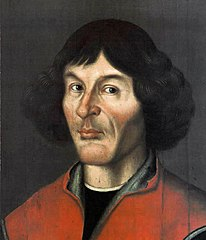
\includegraphics[width=8.3cm]{Nikolaus_Kopernikus} \caption{one column figure}\label{fig:unnamed-chunk-2}
\end{figure}

\subsubsection{TWO-COLUMN FIGURES}

You can also include a larger figure.

\begin{figure}
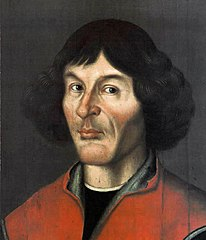
\includegraphics[width=12cm]{Nikolaus_Kopernikus} \caption{two column figure}\label{fig:unnamed-chunk-3}
\end{figure}

\subsection{TABLES}

You can ad \LaTeX table in an R Markdown document to meet the template
requirements.

\subsubsection{ONE-COLUMN TABLE}

\begin{table}[t]
\caption{TEXT}
\begin{tabular}{l c r}
\tophline

a & b & c \\
\middlehline
1 & 2 & 3 \\

\bottomhline
\end{tabular}
\belowtable{Table Footnotes}
\end{table}

\subsubsection{TWO-COLUMN TABLE}

\begin{table*}[t]
\caption{TEXT}
\begin{tabular}{l c r}
\tophline

a & b & c \\
\middlehline
1 & 2 & 3 \\

\bottomhline
\end{tabular}
\belowtable{Table footnotes}
\end{table*}

\subsection{MATHEMATICAL EXPRESSIONS}

All papers typeset by Copernicus Publications follow the math
typesetting regulations given by the IUPAC Green Book (IUPAC:
Quantities, Units and Symbols in Physical Chemistry, 2nd Edn., Blackwell
Science, available at:
http://old.iupac.org/publications/books/gbook/green\_book\_2ed.pdf,
1993).

Physical quantities/variables are typeset in italic font (t for time, T
for Temperature)

Indices which are not defined are typeset in italic font (x, y, z, a, b,
c)

Items/objects which are defined are typeset in roman font (Car A, Car B)

Descriptions/specifications which are defined by itself are typeset in
roman font (abs, rel, ref, tot, net, ice)

Abbreviations from 2 letters are typeset in roman font (RH, LAI)

Vectors are identified in bold italic font using \vec{x}

Matrices are identified in bold roman font

Multiplication signs are typeset using the LaTeX commands
\texttt{\textbackslash{}times} (for vector products, grids, and
exponential notations) or \texttt{\textbackslash{}cdot}

The character * should not be applied as mutliplication sign

\subsection{EQUATIONS}

\subsubsection{Single-row equation}

Unnumbered equations (i.e.~using \texttt{\$\$} and getting inline
preview in RStudio) are not supported by Copernicus.

\begin{equation}
1 \times 1 \cdot 1 = 42
\end{equation}

\begin{equation}
A = \pi r^2
\end{equation}

\begin{equation}
x=\frac{2b\pm\sqrt{b^{2}-4ac}}{2c}.  
\end{equation}

\subsubsection{Multiline equation}

\begin{align}
& 3 + 5 = 8\\
& 3 + 5 = 8\\
& 3 + 5 = 8
\end{align}

\subsection{MATRICES}

\[
\begin{matrix}
x & y & z\\
x & y & z\\
x & y & z\\
\end{matrix}
\]

\subsection{ALGORITHM/PROGRAMMING CODE}

If you want to use algorithms, you need to make sure yourself that the
\LaTeX packages \texttt{algorithms} and \texttt{algorithmicx} are
installed so that \texttt{algorithm.sty} respectively
\texttt{algorithmic.sty} can be loaded by the Copernicus template. Both
need to be available through your preferred \LaTeX{} distribution. With
TinyTeX (or TeX Live), you can do so by running
\texttt{tinytex::tlmgr\_install(c("algorithms",\ "algorithmicx"))}

Copernicus staff will no accept any additional packages from your LaTeX
source code, so please stick to these two acceptable packages. They are
needed to use the example below

\begin{algorithm}
\caption{Algorithm Caption}
\label{a1}
\begin{algorithmic}
\STATE $i\gets 10$
\IF {$i\geq 5$} 
        \STATE $i\gets i-1$
\ELSE
        \IF {$i\leq 3$}
                \STATE $i\gets i+2$
        \ENDIF
\ENDIF
\end{algorithmic}
\end{algorithm}

\subsection{CHEMICAL FORMULAS AND REACTIONS}

For formulas embedded in the text, please use
\texttt{\textbackslash{}chem\{\}}, e.g.~\chem{A \rightarrow B}.

The reaction environment creates labels including the letter R,
i.e.~(R1), (R2), etc.

\begin{itemize}
\item
  \texttt{\textbackslash{}rightarrow} should be used for normal
  (one-way) chemical reactions
\item
  \texttt{\textbackslash{}rightleftharpoons} should be used for
  equilibria
\item
  \texttt{\textbackslash{}leftrightarrow} should be used for resonance
  structures
\end{itemize}

\begin{reaction}
A \rightarrow B \\
\end{reaction}
\begin{reaction}
Coper \rightleftharpoons nicus \\
\end{reaction}
\begin{reaction}
Publi \leftrightarrow cations
\end{reaction}

\subsection{PHYSICAL UNITS}

Please use \texttt{\textbackslash{}unit\{\}} (allows to save the
math/\texttt{\$} environment) and apply the exponential notation, for
example \(3.14\,\unit{km\,h^{-1}}\) (using LaTeX mode:
\texttt{\textbackslash{}(\ 3.14\textbackslash{},\textbackslash{}unit\{...\}\ \textbackslash{})})
or \unit{0.872\,m\,s^{-1}} (using only
\texttt{\textbackslash{}unit\{0.872\textbackslash{},m\textbackslash{},s\^{}\{-1\}\}}).

\conclusions[Conclusions]

The conclusion goes here. You can modify the section name with
\texttt{\textbackslash{}conclusions{[}modified\ heading\ if\ necessary{]}}.



\codedataavailability{use this to add a statement when having data sets
and software code
available} %% use this section when having data sets and software code available

\sampleavailability{use this section when having geoscientific samples
available} %% use this section when having geoscientific samples available

\videosupplement{use this section when having video supplements
available} %% use this section when having geoscientific samples available

%%%%%%%%%%%%%%%%%%%%%%%%%%%%%%%%%%%%%%%%%%
%% optional

%%%%%%%%%%%%%%%%%%%%%%%%%%%%%%%%%%%%%%%%%%
\appendix
\section{Figures and tables in appendices}

Regarding figures and tables in appendices, the following two options
are possible depending on your general handling of figures and tables in
the manuscript environment:

\subsection{Option 1}

If you sorted all figures and tables into the sections of the text,
please also sort the appendix figures and appendix tables into the
respective appendix sections. They will be correctly named
automatically.

\subsection{Option 2}

If you put all figures after the reference list, please insert appendix
tables and figures after the normal tables and figures.

To rename them correctly to A1, A2, etc., please add the following
commands in front of them: \texttt{\textbackslash{}appendixfigures}
needs to be added in front of appendix figures
\texttt{\textbackslash{}appendixtables} needs to be added in front of
appendix tables

Please add \texttt{\textbackslash{}clearpage} between each table and/or
figure. Further guidelines on figures and tables can be found below.
\noappendix

%%%%%%%%%%%%%%%%%%%%%%%%%%%%%%%%%%%%%%%%%%
\authorcontribution{Daniel wrote the package. Josiah thought about
poterry. Markus filled in for a second author.} %% optional section

%%%%%%%%%%%%%%%%%%%%%%%%%%%%%%%%%%%%%%%%%%
\competinginterests{The authors declare no competing
interests.} %% this section is mandatory even if you declare that no competing interests are present

%%%%%%%%%%%%%%%%%%%%%%%%%%%%%%%%%%%%%%%%%%
\disclaimer{We like Copernicus.} %% optional section

%%%%%%%%%%%%%%%%%%%%%%%%%%%%%%%%%%%%%%%%%%
\begin{acknowledgements}
Thanks to the rticles contributors!
\end{acknowledgements}

%% REFERENCES
%% DN: pre-configured to BibTeX for rticles

%% The reference list is compiled as follows:
%%
%% \begin{thebibliography}{}
%%
%% \bibitem[AUTHOR(YEAR)]{LABEL1}
%% REFERENCE 1
%%
%% \bibitem[AUTHOR(YEAR)]{LABEL2}
%% REFERENCE 2
%%
%% \end{thebibliography}

%% Since the Copernicus LaTeX package includes the BibTeX style file copernicus.bst,
%% authors experienced with BibTeX only have to include the following two lines:
%%
\bibliographystyle{copernicus}
\bibliography{rapidfire.bib}
%%
%% URLs and DOIs can be entered in your BibTeX file as:
%%
%% URL = {http://www.xyz.org/~jones/idx_g.htm}
%% DOI = {10.5194/xyz}


%% LITERATURE CITATIONS
%%
%% command                        & example result
%% \citet{jones90}|               & Jones et al. (1990)
%% \citep{jones90}|               & (Jones et al., 1990)
%% \citep{jones90,jones93}|       & (Jones et al., 1990, 1993)
%% \citep[p.~32]{jones90}|        & (Jones et al., 1990, p.~32)
%% \citep[e.g.,][]{jones90}|      & (e.g., Jones et al., 1990)
%% \citep[e.g.,][p.~32]{jones90}| & (e.g., Jones et al., 1990, p.~32)
%% \citeauthor{jones90}|          & Jones et al.
%% \citeyear{jones90}|            & 1990


\end{document}
